\chapter{Perspektivering}
I 2007 blev en fremtidig plan fremlagt for landets hospitaler. Her var målet at skære ned på antallet af hospitaler, der har akutmodtagelse døgnet rundt. Antallet skulle gå fra 40 hospitaler i 2007 til 21 hospitaler i 2020. Denne strukturændring skal give færre og mere specialiserede hospitaler, hvilket skal gøre behandlingen bedre og mere effektiv for de danske borgere. Dette betyder, at der bliver en større afstand mellem hospitalerne, da de mindre hospitaler i provinserne lukker \cite{supersygehus}. Dette giver mere transport for borgerne ved rutinemæssige undersøgelser, blandt andet ultralydsscanning af gravide. Her vil Ultralyds Robotarmen fremtidsmæssigt have et potentiale som en telemedicinsk løsning, hvor problemstillingen med store afstande fjernes. Ultralyds Robotarmen vil også kunne afhjælpe situationen i Grønland, hvor der er endnu større afstand mellem borger og hospital \cite{greenland}.

Den telemedicinske udgave af Ultralyds Robotarmen vil imødekomme økonomiske, organisatoriske, samfundsmæssige og patientrelaterede udfordringer. Her vil Ultralyds Robotarmen blive udstyret med kameraer og en mikrofon, som skal transmittere billede og lyd, se Bilag 12, 28.04.2016. Sonografen vil via joysticket kunne scanne den gravide fra afstand. Figur \ref{systemTelemedicin} viser sammenhængen mellem systemets dele ved den telemedicinske udgave. Sonografen behøver derfor ikke at være placeret i samme rum. Ved den gravide skal der være en assistent til stede, som skal klargøre systemet og forberede scanningen.

\begin{figure}[H]\centering
	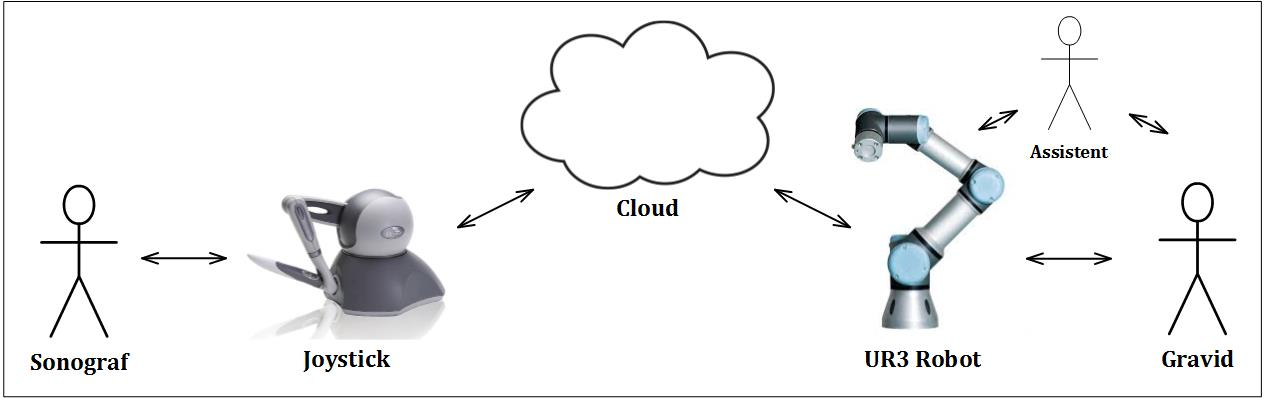
\includegraphics[width = 1.0\textwidth]{Figurer/teknologiTelemedicin.jpg}
	\caption{Sammenhæng mellem systemets dele ved ændring til en telemedicinsk robotarm.}
	\label{systemTelemedicin}
\end{figure}

I Grønland er der få steder, hvor ultralydsscanninger kan udføres og derved store afstande mellem de gravide og sonograferne. Her vil den telemedicinske udgave bevirke, at en sonograf i Danmark, eller et andet sted i Grønland, kan foretage scanningen på gravide placeret afsides steder i Grønland. Dette vil give besparinger på transportudgifter, da patienterne såvel som sonograferne, ikke længere skal transporteres over store afstande ved de rutinemæssige scanninger, se Bilag 12, 18.02.2016. 
Dette vil ligeledes være til gavn i Danmark, hvor ultralydsscanninger vil kunne blive udført i provinserne, selvom sonograferne er placeret i de større byer. Derfor er der potentiale både internationalt og nationalt, da sonografen fra sin egen afdeling vil kunne tilbyde sin ekspertise på tværs af afdelingerne på landets hospitaler. 

Ultralyds Robotarmen som telemedicinsk udgave underbygges af studier, som har undersøgt brugen af ultralyds robotarme som telemedicinske løsninger. Studierne inden for telemedicinsk ultralydsscanning har været i gang i en årrække. Studierne undersøger, hvorvidt det er muligt at få samme kvalitet på telemedicinske scanninger som ved manuelle scanninger. Det undersøges, om billedkvaliteten forbliver den samme, når data skal sendes over internettet. Yderligere undersøges det, om den telemedicinske scanning kan foretages tilfredsstillende \cite{8}\cite{5}\cite{18}\cite{Hjerterobot}. 





